\documentclass[a4paper,12pt]{report}

% Packages
\usepackage[utf8]{inputenc}  % Encoding
\usepackage{amsmath}         % Math symbols
\usepackage{amssymb}         % Additional math symbols
\usepackage{graphicx}        % Images
\usepackage[hidelinks]{hyperref}
\usepackage{caption}         % Captions
\usepackage{geometry}        % Page layout
\geometry{a4paper, margin=0.8in}
\usepackage{setspace}        % Line spacing
\usepackage{titlesec}        % Title customization
\usepackage{float}
\usepackage{listings}        % Code formatting
\usepackage{xcolor}
\usepackage{tabularx}
\usepackage{booktabs} % For better table lines
\usepackage{array}
\usepackage{makecell}

% Customization
\setcounter{secnumdepth}{3}  % Section numbering depth
\setcounter{tocdepth}{3}     % Table of contents depth
\setlength{\parindent}{0pt}
\renewcommand{\baselinestretch}{1.5}  % Line spacing
\renewcommand{\lstlistingname}{Code}
\renewcommand{\lstlistlistingname}{List of Code Blocks }


% Define Code Block Style
\lstdefinestyle{mystyle}{
    commentstyle=\color{gray},
    keywordstyle=\bfseries,
    basicstyle=\ttfamily\footnotesize, % Change font to Courier New
    breaklines=true,                   
    captionpos=b,                      
    keepspaces=true,                   
    numbers=left,                      
    numbersep=5pt,                     
    numberstyle=\tiny\color{gray},     
    showspaces=false,                  
    showstringspaces=false,            
    showtabs=false,                    
    tabsize=4,
    frame=single % Clean single-line frame
}

% Apply the style globally
\lstset{style=mystyle}
\title{\textbf{Smart Home Automation}}
\author{Your Name}
\date{\today}

\begin{document}
\begin{titlepage}
    \centering

    {\Huge \textbf{Smart Home Automation}}\\[0.5cm]
    {\Large \textit{Major Project Report}}\\[1.5cm]

    
\includegraphics[width=0.4\textwidth]{nitkkr.png}\\[1cm] % Replace nitkkr.png with the actual path to your logo file.

    \textbf{\Large National Institute of Technology, Kurukshetra}\\[1cm]
    
    \begin{minipage}[t]{0.45\textwidth}
        \raggedright
        \textbf{\large Submitted By:}\\
        {\Large \textbf{Armaan Dhillon}}\\
        {\large Roll No: 12114058}\\
        {\large Department of Electrical Engineering}\\
    \end{minipage}
    \hfill
    \begin{minipage}[t]{0.45\textwidth}
        \raggedleft
        \textbf{\large Submitted To:}\\
        {\Large \textbf{Dr. Monika Mittal}}\\
        {\large Department of Electrical Engineering}\\
    \end{minipage}

    \vfill

    {\large January 2025 - May 2025}
\end{titlepage}

% ---------------------- CANDIDATE DECLARATION ----------------------
\begin{center}
    \textbf{Electrical Engineering Department}\\
    \textbf{National Institute of Technology Kurukshetra}\\[1cm]
    
    \textbf{\Large CANDIDATE DECLARATION}\\
    \hrulefill
\end{center}

\vspace{0.5cm}

I hereby declare that the work presented in this report,  
\textbf{“Smart Home Automation”}, is an original work that was completed under the supervision of \textbf{Dr. Monika Mittal} and submitted to the  
\textbf{Department of Electrical Engineering}. 

I have not submitted the work described in this dissertation for the grant of any other degree from this or any other institute. I have respected intellectual property rights in every possible way and have assisted others in using them for academic purposes.  

I shall be held responsible for any complete or partial copyright violation or intellectual property rights violation discovered at any time after the award of my degree, and not my Supervisor/Head of the Department/Institute.

\vspace{2cm}

\noindent
\begin{flushright}
Armaan Dhillon  \hspace{3cm} \\ 
12114058  \hspace{3cm} \\ 
\end{flushright}

\newpage

% ---------------------- CERTIFICATE ----------------------
\begin{center}
    \textbf{Electrical Engineering Department}\\
    \textbf{National Institute of Technology Kurukshetra}\\[1cm]
    
    \textbf{\Large CERTIFICATE}\\
    \hrulefill
\end{center}

\vspace{0.5cm}

Certified that the work described by Mr. \textbf{Armaan Dhillon} (Roll No. \textbf{12114058}), \textbf{“Smart Home Automation”},was completed under my supervision during the \textbf{8th Semester}. According to our knowledge, this work has not been submitted for a degree elsewhere.

\vspace{6cm}

\begin{flushright}
\textbf{Dr. Monika Mittal}\\
Associate Professor\\
NIT Kurukshetra
\end{flushright}

\newpage

% ---------------------- ACKNOWLEDGMENTS ----------------------
\begin{center}
    \textbf{\Large ACKNOWLEDGMENTS}\\
    \hrulefill
\end{center}

\vspace{0.5cm}

My heartfelt gratitude goes out to my supervisor, \textbf{Dr. Monika Mittal}, for her helpful assistance and unwavering support throughout this project. Her technical expertise, accurate recommendations, and timely guidance were invaluable. Her wisdom and insight provided me with a great deal of motivation.  

Additionally, I would like to express my sincere gratitude to \textbf{Prof. B.V. Rama Reddy}, Director of NIT Kurukshetra, and \textbf{Prof. Jyoti Ohri}, Head of the Department, for creating a conducive environment and inspiring us to pursue constructive research efforts.  

I also want to express my gratitude to all the instructors and staff at the NIT Kurukshetra Electrical Engineering Department for their invaluable assistance and support.  

I would like to extend my sincere gratitude to my colleagues and seniors for their valuable suggestions and encouragement, which helped me complete my thesis work.

\begin{abstract}
    Home automation utilizing Raspberry Pi has grown in popularity due to its low cost and capacity to improve convenience and energy efficiency.  However, many existing home automation systems suffer severe issues, such as inadequate security, restricted interoperability, lengthy configuration processes, and insufficient real-time energy monitoring.  This project overcomes these restrictions by creating a smart home automation system that combines Raspberry Pi, ThingsBoard, Docker, and real-time sensor data to deliver a safe, modular, and scalable solution.
    
    The system collects energy usage data from sensors linked to a smart energy meter and delivers it to a cloud-based IoT platform using MQTT and REST APIs.  ThingsBoard enables real-time visualization and control via customisable dashboards, while Docker ensures modular deployment and service separation.  The use of encrypted communication protocols improves security, while the open-source, protocol-agnostic architecture allows for smooth integration of numerous devices.  This project provides a realistic and efficient solution to modern home automation by simplifying system setup and enabling real-time monitoring and automation, resulting in improved energy management and user accessibility.
\end{abstract}
    

\tableofcontents
\listoffigures
\newpage
\chapter{Introduction}
\section{Introduction}
Home automation using Raspberry Pi has gained popularity due to its numerous advantages and cost-effectiveness. These systems provide users with the ability to control household appliances through local networks or remote access, thereby enhancing convenience and energy efficiency\cite{jain2014raspberry}. Modern home automation technologies offer features such as automatic meter reading, real-time monitoring, and remote control of electrical connections without the need for personal involvement\cite{chaudhari2017smart}. In addition to energy monitoring, home automation systems commonly include sensors, cameras, and web-based applications to increase security and enable comprehensive device control\cite{patchava2015smart}. The MQTT protocol, known for its lightweight and reliable messaging, is frequently used in IoT-based systems to improve data quality and communication reliability\cite{Atmoko_2017}.

Despite these developments, there are still certain limits in existing home automation options. Many systems continue to have insufficient encryption and access control, leaving them vulnerable to illegal access. Proprietary communication protocols and restricted integration possibilities further impede interoperability across devices from different manufacturers. Furthermore, extensive setup processes and non-intuitive user interfaces make it difficult for non-technical individuals to access and operate.

This project addresses these challenges by creating a smart home automation system using Raspberry Pi, Docker, ThingsBoard, and real-time sensor data. The use of encrypted MQTT assures safe communication, while Docker containers enable modular deployment and service isolation. ThingsBoard supports protocol-agnostic integration and user-friendly dashboards, easing system maintenance and customization. The system's real-time monitoring and automation aims to increase energy efficiency, user experience, and support for a scalable, cost-effective, and open-source approach to home automation.

\section{Problem Statement}

Smart home automation has received a lot of interest in recent years because of its ability to improve energy efficiency, increase convenience, and enable cognitive management over household appliances. Despite significant development in this area, current systems suffer a number of ongoing problems that restrict their effectiveness and widespread acceptance.

One of the primary considerations is security. Existing systems frequently use inadequate encryption standards and lack effective access control measures. This makes the system susceptible to unwanted access, data breaches, and manipulation of essential home systems. Furthermore, interoperability presents a substantial challenge. Many commercial smart home solutions use proprietary communication protocols and closed designs, making it impossible to integrate devices from other suppliers or expand the system without encountering compatibility concerns.

Another important factor to consider is user experience. Many smart home systems are difficult to set up and provide little customization, discouraging non-technical consumers from embracing and efficiently utilizing new technologies. Finally, energy efficiency remains a significant concern in many systems. Limited support for real-time monitoring and control of energy consumption frequently leads to wasteful power consumption and higher operational costs.

\section{Proposed Solution}

To overcome these issues, a smart home automation solution was created that combines Raspberry Pi, ThingsBoard, Docker, and real-time sensor data. This system seeks to be affordable, secure, flexible, and adaptable to a wide range of residential situations.

The Raspberry Pi is the primary hardware platform, operating as a local controller and managing edge computing duties. It supports sensor data gathering and communication with connected devices. ThingsBoard, an open-source IoT platform, is used for device administration, real-time data visualization, and building interactive dashboards. This platform supports several protocols and enables for simple customisation, addressing interoperability and user experience issues.

Docker uses containerization to isolate services, improve system security, and simplify deployment and upgrades. Each service operates in its own container, making the system more flexible and simple to manage or scale. Real-time sensor integration enables continuous monitoring of environmental conditions and energy consumption, resulting in automation and increased energy efficiency.

From a security standpoint, encrypted MQTT protocols are employed for data transmission, establishing a safe communication channel between devices and the cloud platform. Docker-based service isolation provides an additional degree of safety, reducing possible risks from system flaws.

In terms of interoperability, the system is intended to be protocol-agnostic and completely open source. This enables the smooth integration of several devices, independent of manufacturer, and encourages vendor independence. To improve the user experience, the platform includes visual dashboards with drag-and-drop widgets, allowing users to design and monitor their smart home environment with little technical knowledge.

Real-time sensor data enables dynamic decision-making, allowing the system to respond immediately to changes in ambient conditions. This improves energy efficiency by enabling context-aware automation, such as changing lighting or shutting off equipment when not in use.

\section{Project Workflow}

This section depicts the workflow of a smart home automation system that is coupled with blockchain for energy billing. The smart meter captures energy usage data, which is then transmitted to a cloud-based IoT platform for real-time monitoring\cite{jain2014raspberry}\cite{chaudhari2017smart}. Data is processed using MQTT and REST APIs to ensure reliability\cite{Atmoko_2017}.

A Web3 application obtains this information and communicates with an Ethereum smart contract to generate energy bills in a secure and transparent manner\cite{10.1145/3328833.3328857}\cite{Hu2018BlockchainbasedSC}. By merging IoT and blockchain, the solution automates billing and payments, increasing efficiency and security.

\subsection{System Architecture}

The architecture consists of multiple interconnected components, including sensors, microcontrollers, cloud platforms, and blockchain technology. The data flow and interactions are illustrated in Figure~\ref{fig:workflow}.

\begin{figure}[h]
    \centering
    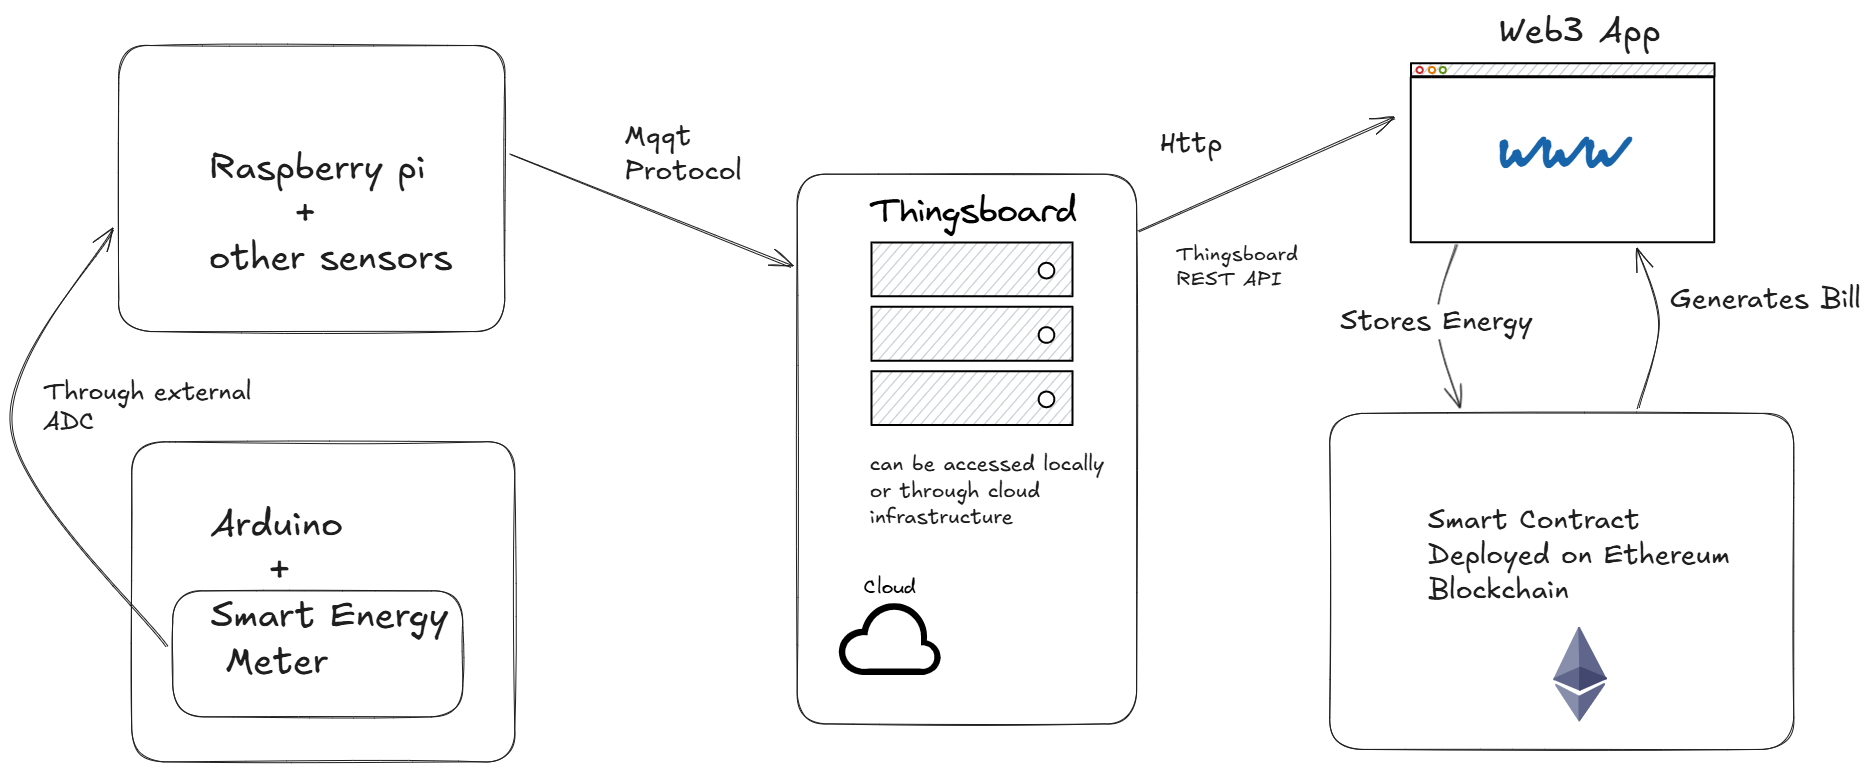
\includegraphics[width=0.9\textwidth]{basicArchitecture.png}
    \caption{System Workflow}
    \label{fig:workflow}
\end{figure}

\subsection{Components and Data Flow}

\paragraph{Energy Measurement and Data Acquisition:} The system starts with an Arduino connected to a smart energy meter, which measures power consumption. Since Arduino lacks a built-in analog-to-digital converter (ADC) with the required resolution, an external ADC is used for accurate readings. The measured data is then transmitted to a Raspberry Pi for further processing.

\paragraph{Data Transmission and Storage:} This section illustrates the workflow of a smart home automation system that is integrated with blockchain for energy billing. The system's goal is to collect energy consumption data, store it in a cloud-based IoT platform, and bill and pay using a Web3 application that interacts with an Ethereum blockchain smart contract.

\paragraph{Web3 Integration and Smart Contracts:} A Web3 application fetches energy consumption data from ThingsBoard via HTTP requests. The retrieved energy data is then stored in a smart contract deployed on the Ethereum blockchain. The smart contract automatically generates an energy bill based on the stored consumption values.

\paragraph{Billing and Payment System:} Using HTTP queries, a Web3 application retrieves energy usage data from ThingsBoard. A smart contract that is implemented on the Ethereum blockchain then stores the energy data that has been recovered. Using the saved consumption values, the smart contract automatically creates an energy bill.

\section{Conclusion}

This process combines blockchain, cloud computing, and the Internet of Things to produce an automated and decentralized energy billing system. An effective and transparent billing procedure is made possible by the modular architecture, which facilitates smooth data flow from energy monitoring to smart contract interactions.

\chapter{Literature Survey}

\section{Introduction}
Smart home automation has become a vital part of modern living, offering benefits such as increased convenience, energy optimization, and enhanced security. With the advancement of Internet of Things (IoT) technologies, homes are now equipped with interconnected sensors, controllers, and cloud platforms that enable real-time automation and monitoring. However, as noted in numerous studies, the journey toward widespread adoption remains hindered by technical, financial, and usability-related challenges \cite{julies}\cite{Zhang2022TheCS}\cite{Ahmed02102021}.

While these technologies show promise, real-world implementations frequently fall short due to constraints such as inadequate device interoperability, security risks, a lack of customisation, and exorbitant installation costs.  Existing systems sometimes rely on closed ecosystems, further complicating integration and limiting user flexibility.  This chapter explores major literature in the field, identifies the primary barriers to smart home automation, and compares those results to our system's implementation, which uses Raspberry Pi, ThingsBoard, Docker, and real-time sensor-cloud connection.



\section{Overview of the Research Domain}
The smart home ecosystem comprises a diverse set of devices and platforms that collaborate to automate household operations.  Temperature control, lighting, security systems, and energy monitoring are all examples of IoT-enabled applications.  As seen in recent studies, the integration of different sensors and platforms brings both functional potential and additional complications\cite{Venkatesh}.

Security breaches, data privacy issues, device incompatibilities, and poor user engagement remain significant impediments to adoption.  Although open-source systems and current edge computing devices such as the Raspberry Pi provide promising possibilities, much of the research focuses on systems that are either highly centralized or dispersed due to proprietary constraints.  This assessment divides the main challenges into four categories: security, interoperability, user experience, and energy efficiency.


\section{Review of Existing Work}
\subsection{Security Concerns}
Security in smart home automation is a serious concern raised in various research.  As the number of internet-connected gadgets grows, so does the attack surface for cyber attacks.  According to multiple sources, many IoT devices lack strong encryption and authentication, leaving them vulnerable to unauthorized access\cite{Venkatesh}\cite{mazid2023iot}.  Others raise worries about user data being collected or modified owing to inadequate or nonexistent privacy protections\cite{li2023let}.  Furthermore, the lack of common security methods across different manufacturers increases these risks\cite{Sobin_2020}\cite{holguin2023smart}.

\subsection{Interoperability Issues}
Interoperability refers to the ability of equipment from various vendors to communicate seamlessly.  According to research, many smart home systems fail to integrate effectively because they use proprietary communication protocols\cite{portales2019challenges}\cite{Sobin_2020}.  Incompatibility between platforms frequently causes users to rely on vendor-specific hubs or apps, resulting in a disjointed user experience.  This difficulty is exacerbated by the lack of globally accepted IoT standards\cite{holguin2023smart}.

\subsection{User Experience}
Despite their functional potential, smart home systems can provide a terrible user experience.  According to studies, setup methods are typically technically complex, preventing non-expert users\cite{sita2024development}\cite{bai2024research}.  Other findings indicate that many systems fail to tailor interactions depending on user behavior, leaving automation seeming stiff and detached\cite{elmi2023interoperable}.  Furthermore, non-intuitive interfaces and a lack of transparency increase user irritation and slow adoption\cite{mare2019consumer}.

\subsection{Energy Efficiency}
Energy efficiency is usually highlighted as a significant motivator for smart home adoption, however research shows that many systems fall short of meeting this expectation.  Several studies address how real-time energy monitoring and management are underutilized due to the high system complexity\cite{sita2024development}.  Others point out that balancing user comfort with energy-saving automation is a continuing challenge\cite{Sobin_2020}\cite{elmi2023interoperable}, and that consumers frequently lack awareness into their own consumption habits\cite{kaur2024evolution}.




\section{Research Gaps and Motivation}
While the present literature thoroughly examines the theoretical and technological underpinnings of smart home automation, the majority of solutions are either too expensive or do not provide end-to-end capability.  Systems that rely significantly on centralized cloud services are vulnerable to latency, data breaches, and platform dependencies.  On the other hand, decentralized systems frequently lack the coordination and integration needed for comprehensive automation.

 The proposed project was motivated by the need for a modular, cost-effective, and fully adaptable system that could be readily installed and maintained.  The project takes a balanced approach, using a Raspberry Pi as an edge controller, ThingsBoard for visualization and device management, and Docker for scalable deployment, to bridge the gap between academic research and real-world applications.

 \section{Comparative Analysis with the Proposed Solution}

The proposed smart home automation solution utilizes Raspberry Pi, ThingsBoard, Docker, and real-time sensor data integration to address limitations identified in existing literature. By leveraging open-source and containerized technologies, it aims to offer a low-cost, secure, and modular framework adaptable to varied use cases. Table~\ref{tab:comparison} summarizes how this solution compares with the challenges found in previous research.

\begin{table}[htbp]
    \centering
    \renewcommand{\arraystretch}{1.5} % Adds vertical padding
    \setlength{\tabcolsep}{8pt}       % Adds horizontal padding
    \begin{tabular}{|>{\centering\arraybackslash}m{3cm}|
                    >{\centering\arraybackslash}m{5.5cm}|
                    >{\centering\arraybackslash}m{5.5cm}|}
    \hline
    \textbf{Challenge} & \textbf{Literature Observations} & \textbf{Proposed Solution} \\
    \hline
    Security & Weak encryption, poor access control & Encrypted MQTT, Docker-based isolation \\
    \hline
    Interoperability & Proprietary protocols, poor integration & Open-source, protocol-agnostic stack \\
    \hline
    User Experience & Complex setup, limited personalization & Visual dashboards, easy configuration \\
    \hline
    Energy Efficiency & Limited real-time monitoring & Live sensor data, extensible dashboards \\
    \hline
    
    \end{tabular}
    \caption{Comparison of Literature Challenges and Proposed Solution}
    \label{tab:comparison}

\end{table}
    

 
\section{Conclusion}
Smart home automation is always evolving, with substantial advances in device capabilities, cloud integration, and automation intelligence.  However, difficulties such as security vulnerabilities, device compatibility, usability, and energy management continue to impede large-scale adoption.  Existing literature identifies these difficulties, but often lacks practical remedies.

This project provides a comprehensive, technically competent response to these difficulties.  It provides a realistic framework that corresponds with academic research concepts while boosting scalability, dependability, and user empowerment by integrating open-source platforms, containerized infrastructure, and real-time sensor-cloud communication.

\chapter{Proteus Schematic Design and Simulation}

\section{Introduction}
Proteus is a powerful software program that is commonly used to develop and simulate embedded systems prior to their real implementation.  It allows you to efficiently test circuits, detect design problems, and enhance performance without the need for actual hardware.  This chapter focuses on the schematic design and modeling of a smart home automation system and a smart energy meter, which integrate sensors, actuators, and communication modules to provide real-time monitoring and control.


The Raspberry Pi 3 serves as the core processing unit for the smart home automation system, which communicates with a variety of sensors such as Light Dependent Resistors (LDR), Passive Infrared (PIR) sensors, and gas detectors to automate household appliances.  The Raspberry Pi lacks built-in analog input capabilities, thus an external ADC (MCP3208) is used to interpret analog sensor data and enabling IoT-based automation\cite{valov2020home}.

The smart energy meter focuses on real-time power consumption monitoring, incorporating an Arduino Uno for data acquisition, ACS712 current sensors for current measurement, and voltage dividers for accurate voltage monitoring \cite{li2010application}. Additionally, power factor measurement is achieved using LM358 operational amplifiers and XOR gates to analyze phase differences between voltage and current waveforms \cite{Khair_2017}. These measurements are transmitted to the IoT platform, enabling remote energy management and optimization.

This chapter details the schematic design, component selection, and software implementation in Proteus.  The proposed system provides not just automation and remote monitoring, but also efficient energy utilization and billing.  Proteus simulations evaluate the system's many features prior to real-world deployment, ensuring reliability and performance.

\section{Schematic Design in Proteus}
\subsection{Smart Home Automation System}
The home automation circuit includes:

\textbf{Raspberry Pi 3:} The Raspberry Pi 3 B+ was chosen for this home automation project because of its powerful capabilities and simplicity of integration.  It is driven by a Broadcom BCM2837B0 quad-core Cortex-A53 (ARMv8) processor clocked at 1.4GHz, with 1GB LPDDR2 SDRAM and a Broadcom Videocore-IV GPU. Networking options include Gigabit Ethernet (by USB), dual-band Wi-Fi (2.4GHz and 5GHz 802.11b/g/n/ac), and Bluetooth 4.2 (BLE)\cite{valov2020home}.It includes a 40-pin GPIO header, HDMI, a 3.5mm audio connector, four USB 2.0 ports, Ethernet, CSI, and DSI.  The Micro-SD storage format and compact dimensions (82mm × 56mm × 19.5mm, 50g) make it ideal for embedded applications\cite{valov2020home}.

\begin{figure}[H]  % 'h' places the figure approximately here
    \centering
    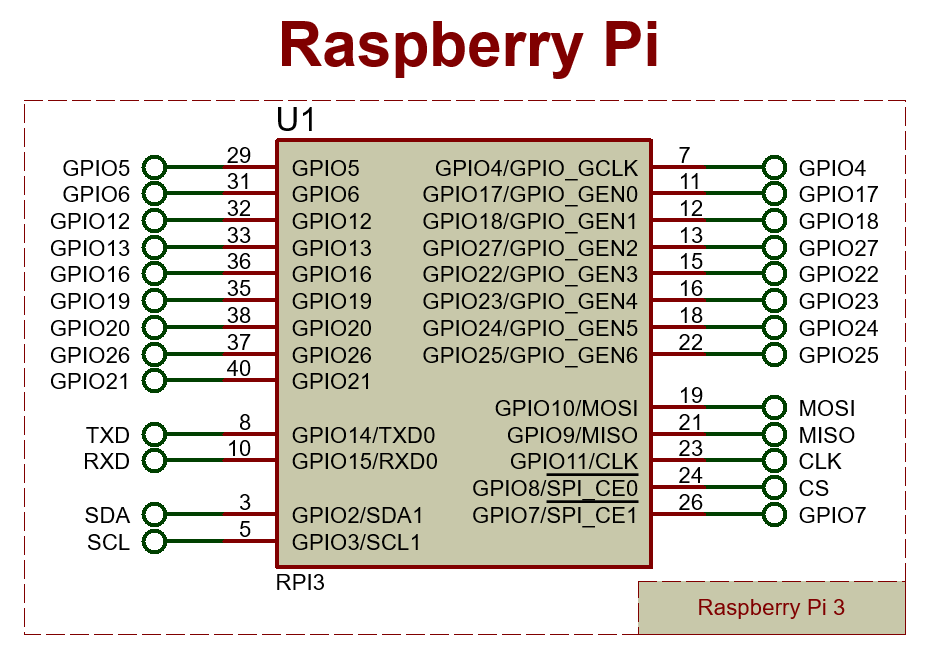
\includegraphics[width=0.6\textwidth]{image.png} % Adjust width as needed
    \caption{Raspberry Pi 3 Schematic}
    \label{fig:Raspberry} % Label for referencing the figure
\end{figure}


\textbf{ADC (MCP3208):} Analog-to-digital converters (ADCs) transform analog signals into digital data, allowing microcontrollers and computers to process real-world inputs.The MCP3208 is a 12-bit ADC with 8 input channels. It provides high accuracy (±1 LSB DNL, ±1-2 LSB INL) and low power consumption.  It runs on 2.7V-5.5V, has an SPI interface, and is commonly used for sensor applications and data gathering\cite{Dout199927V41}.

\begin{figure}[H]  % 'h' places the figure approximately here
    \centering
    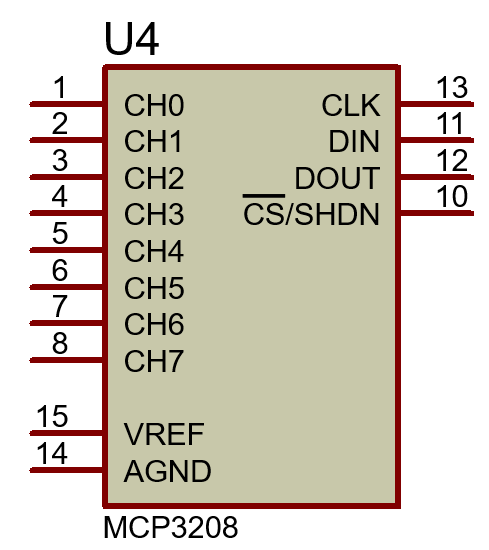
\includegraphics[scale=0.4]{MCP3208.PNG} % Adjust width as needed
    \caption{ADC (MCP3208)}
    \label{fig:adc} % Label for referencing the figure
\end{figure}

Because Raspberry Pi lacks built-in analog inputs, an external ADC such as the MCP3208 is required to read analog sensor data.  Interfacing via SPI allows for real-time monitoring in IoT applications and industrial automation\cite{Flurry2021}.

\textbf{Other Sensors:} We used a variety of sensors and actuators to allow for sophisticated control and monitoring.  The system uses an LDR (Light Dependent Resistor) to detect ambient light levels, allowing lights to be turned on or off based on the brightness of the surroundings. 
A PIR (Passive Infrared) sensor was used to detect motion and human presence.  This sensor is essential for security and automated lighting because it activates lights or alerts when motion is detected.  Furthermore, a MQ-2 gas sensor was used to monitor air quality and identify combustible gases such as LPG and CO, assuring safety by sending alarms in the event of a gas leak.  The LM35 temperature sensor was included to properly monitor room temperature and allow for automatic cooling control.

\subsection{Complete Schematic of Smart Home Automation System}
The smart home automation circuit integrates multiple sensors and actuators to automate home appliances based on environmental conditions ans involves following connections.
\begin{figure}[H]  % 'h' places the figure approximately here
    \centering
    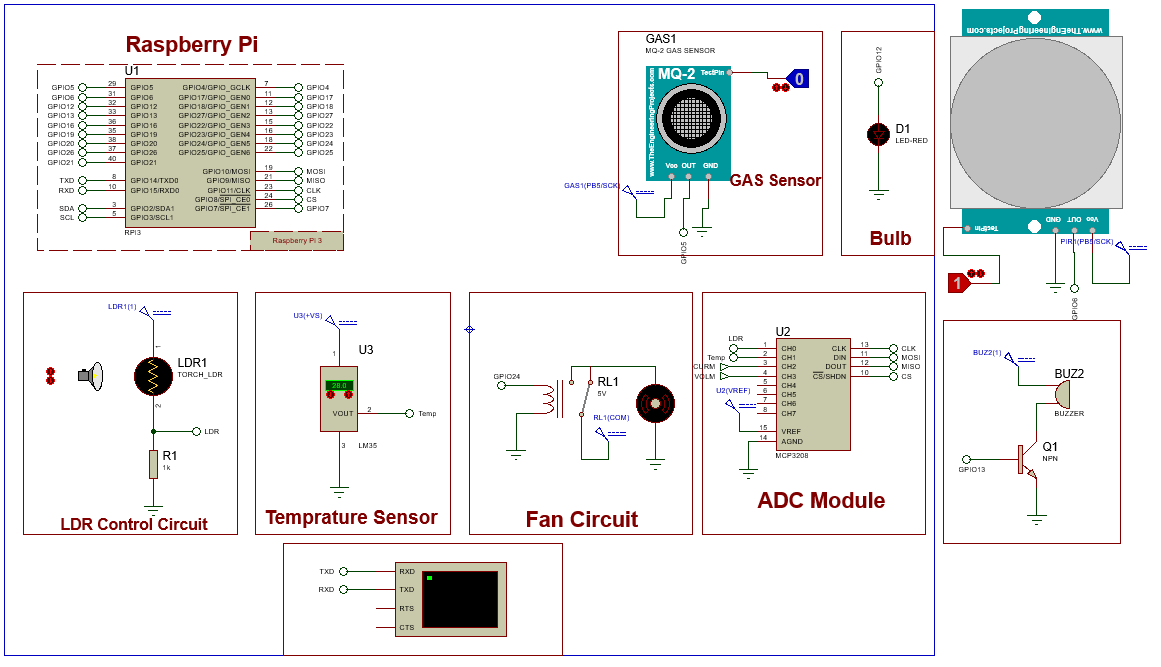
\includegraphics[scale=0.68]{smartHomeAutocomplete.PNG} % Adjust width as needed
    \caption{Complete Schematic}
    \label{fig:schematichome} % Label for referencing the figure
\end{figure}



\subsection{Smart Energy Meter and Power Factor Measurement}
The smart energy meter circuit consists of:

\textbf{Arduino Uno:}The Arduino Uno, built around the AVR microcontroller, has developed as a versatile platform for teaching and implementing digital control systems.  


\begin{figure}[H]
    \centering
    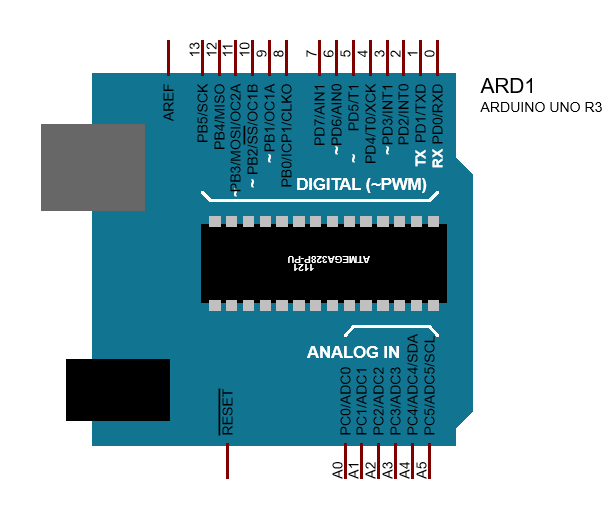
\includegraphics[width=0.6\textwidth]{Capture.PNG} % Adjust width as needed
    \caption{Arduino Uno}
    \label{fig:uno} % Label for referencing the figure

\end{figure}
It has characteristics suited for power electronics applications, providing switching frequencies of up to 100 kHz with extra libraries\cite{muller2015using}.  The Arduino Uno has been shown to be effective in controlling industrial-scale instruments, performing similarly to industrial-class controllers that use PID algorithms\cite{Taufiq_2020}.The Arduino Uno, which is based on the Atmega328 processor, supports Assembly and C programming, allowing students to learn about microcontroller architecture and interact with real-world devices like LCDs, motors, and sensors\cite{Naimi2017TheAM}. 

\textbf{Current Measurement}:In our smart home automation project, we employ the ACS712 Hall-effect-based current sensor to monitor AC/DC power levels. It has low resistance (1.2 mohm) and 2.1 kVRMS isolation for precise and safe current measuring\cite{li2010application}. The 30A variant with 66mV/A sensitivity is integrated with an arduino uno, allowing for real-time power tracking and energy consumption analysis via ThingsBoard.  Calibration improves accuracy and reduces measurement error, making it ideal for IoT-based billing and automation systems.  Its rapid reaction (5 µs) and low noise improve performance for smart energy management\cite{Khair_2017}.
\begin{figure}[H]
    \centering
    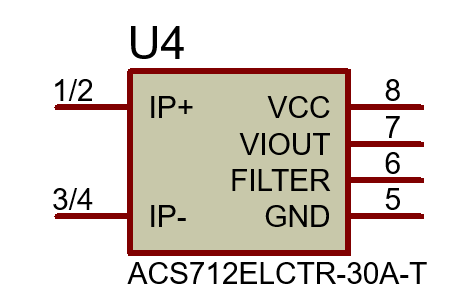
\includegraphics[width=0.35\textwidth]{ACS.PNG} % Adjust width as needed
    \caption{Current Sensor}
\end{figure}


\textbf{Voltage Measurement:}We monitor AC voltage in our smart home automation project with a step-down transformer, a voltage divider network, and a filtering capacitor. The step-down transformer (TR3) converts the high AC mains voltage to a lower, safer level suited for measurement. The voltage divider circuit (R9, R10, R11, and R12) reduces the voltage to a range compatible with the Arduino ADC, ensuring precise readings while protecting the microcontroller. A 500µF capacitor (C2) filters, reduces noise, and stabilizes the signal for accurate RMS voltage measurement. This configuration enables the Arduino to process voltage data and send it to ThingsBoard, allowing for real-time monitoring and effective energy management in our smart home system.
\begin{figure}[H]
    \centering
    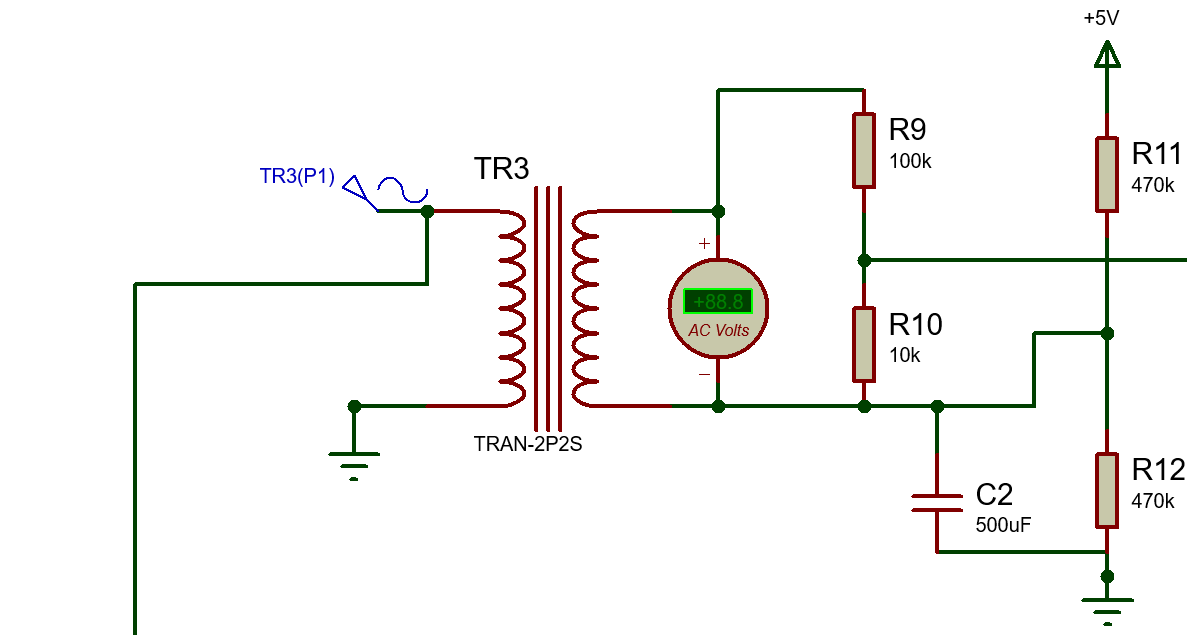
\includegraphics[width=0.6\textwidth]{voltageMeasurment.PNG} % Adjust width as needed
    \caption{Voltage Measurement Circuit}
\end{figure}

\textbf{Power Factor Measurement:} we monitor power factor with LM358 operational amplifiers and an XOR gate.  The LM358 op-amps act as zero-crossing detectors, transforming AC voltage and current waveforms to square waves.  The first op-amp (U8:A) detects zero crossings in the voltage waveform, whereas the second op-amp (U8:B) detects current waveform.  These processed signals are then routed through an XOR gate (U9), which generates a pulse-width output proportional to the phase difference between the voltage and current waves.  The Arduino measures pulse width and calculates power factor as cos($\theta$), where $\theta$ is the phase angle.
\begin{figure}[h]
    \centering
    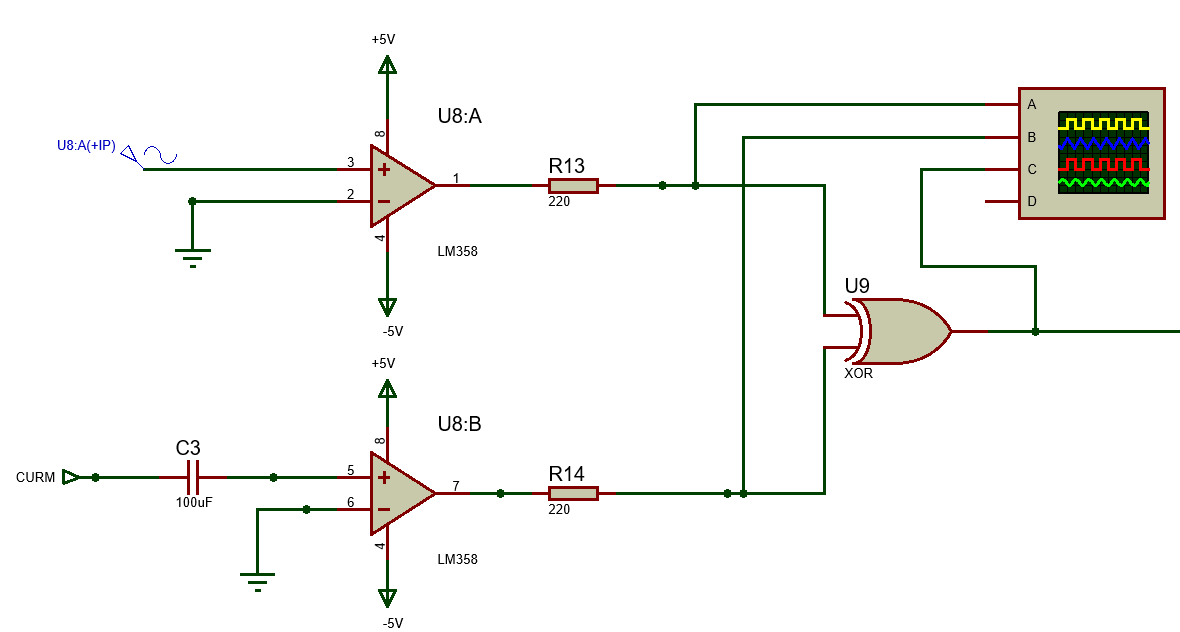
\includegraphics[width=0.6\textwidth]{PowerFactor.PNG} % Adjust width as needed
    \caption{PowerFactor Measurement Circuit}
\end{figure}

\textbf{relay-based load control} electrical appliances are managed remotely using a relay control system. The circuit consists of electromagnetic relays (RL4, RL5) that are controlled by the microcontroller's GPIO pins (for example, Raspberry Pi or Arduino). When a GPIO pin is set to HIGH, the accompanying relay coil is activated, shutting the switch and enabling current to flow to the attached load (such as lights or motors).

\subsection{Complete Schematic of Smart Energy Meter}
The smart energy meter circuit is designed to measure and monitor power consumption while ensuring efficient energy usage.
\begin{figure}[H]
    \centering
    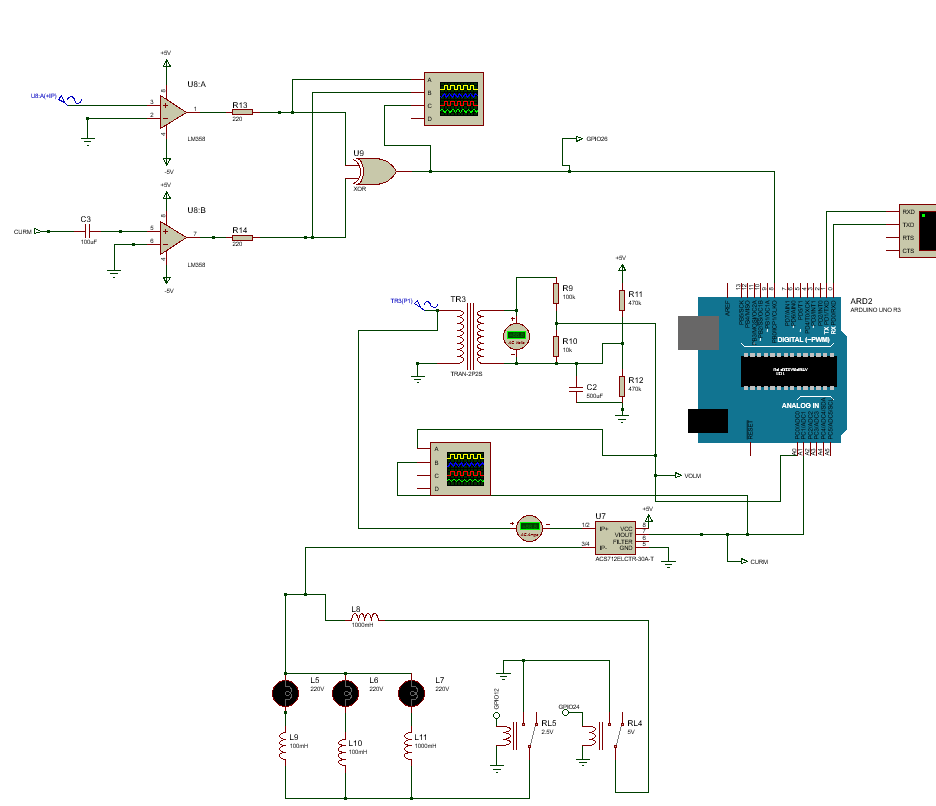
\includegraphics[width=1\textwidth]{smartEnergy.PNG} % Adjust width as needed
    \caption{Complete Schematic of Smart Energy meter}
\end{figure}

\section{Code Implementation}

\subsection{Arduino Code for Smart Energy Meter}

The Arduino is responsible for measuring voltage, current, and calculating power consumption in real-time. The analog pins read voltage and current sensor outputs, which are then converted into meaningful electrical values. The calculated power is then transmitted over serial communication.
\clearpage

\begin{lstlisting}[language=C,caption={arduino code for energy calculations}]
// Pin configuration
const int voltagePin = A0; // Voltage sensor input
const int currentPin = A1; // Current sensor input

// Constants for sensor calibration
const float voltageMultiplier = 230.0 / 1023.0;  // Adjust based on sensor specs
const float currentMultiplier = 10.0 / 1023.0;   // Adjust for CT sensor scaling

void setup() {
    Serial.begin(9600);  // Start serial communication
}

void loop() {
    // Read raw analog values from sensors
    int rawVoltage = analogRead(voltagePin);
    int rawCurrent = analogRead(currentPin);
    
    // Convert raw values to real-world measurements
    float voltage = rawVoltage * voltageMultiplier;
    float current = rawCurrent * currentMultiplier;
    float power = voltage * current; // Active power calculation

    // Print the measurements to serial monitor
    Serial.print("Voltage: "); Serial.print(voltage); Serial.print(" V, ");
    Serial.print("Current: "); Serial.print(current); Serial.print(" A, ");
    Serial.print("Power: "); Serial.print(power); Serial.println(" W");

    delay(1000);  // Wait 1 second before next reading
}
\end{lstlisting}


\subsection{Raspberry Pi Code for Home Automation}

The Raspberry Pi is responsible for reading sensor data, controlling home appliances based on environmental conditions, and sending data to an IoT platform (ThingsBoard) using MQTT.
\clearpage

\begin{lstlisting}[language=Python,caption={Raspberry Pi Code Collects Sensor Data and Sends it over using MQTT}]
import RPi.GPIO as GPIO
import time
import json
import spidev
import math
from paho.mqtt.client import Client

# GPIO setup
GPIO.setmode(GPIO.BCM)
GPIO.setup(17, GPIO.IN)  # LDR sensor for light detection
GPIO.setup(27, GPIO.OUT) # Relay control for light switching

# SPI setup for ADC communication (e.g., MCP3008)
spi = spidev.SpiDev()
spi.open(0, 0)
spi.max_speed_hz = 1350000

# MQTT setup
THINGSBOARD_HOST = "localhost"
ACCESS_TOKEN = "your_access_token"
client = Client()
client.username_pw_set(ACCESS_TOKEN)
client.connect(THINGSBOARD_HOST, 1883, 60)

# Read ADC channel for sensor values
def read_channel(channel):
    adc = spi.xfer2([1, (8 + channel) << 4, 0])
    return ((adc[1] & 3) << 8) + adc[2]

# Calculate RMS voltage from multiple samples
def calculate_rms_voltage():
    sum_squares = sum((read_channel(3) * 3.3 / 1023.0) ** 2 for _ in range(200))
    return math.sqrt(sum_squares / 200) * 11  # Voltage divider correction

# Publish sensor data to MQTT
def publish_sensor_data():
    while True:
        light_level = read_channel(0)  # Read LDR sensor value
        GPIO.output(27, light_level < 100)  # Turn on relay if dark
        
        payload = json.dumps({
            "light": light_level,
            "voltage": calculate_rms_voltage()
        })
        client.publish("v1/devices/me/telemetry", payload)
        time.sleep(0.5)  # Wait before next update

publish_sensor_data()
\end{lstlisting}

\section{Simulation and Testing}

\subsection{Home Automation Testing}
Several tests were run in the Proteus simulation environment to validate the smart home automation system.  The LDR-based light control circuit was tested under various lighting situations.  The simulation confirmed that when the light intensity fell below a particular threshold, the relay was activated, which turned on the linked bulb.  When the light intensity increased, the relay deactivated and the bulb turned off.  This behavior provided automatic lighting management based on ambient light levels.

 The PIR sensor was tested by mimicking motion within its detecting range.  When motion was detected, the buzzer sounded an alert.  When there was no motion, the buzzer remained off.  This proved that the motion detection system was working properly, making it appropriate for security applications.


The MQTT communication between the Raspberry Pi and ThingsBoard Cloud was also tested. Sensor data, including light intensity and relay state, was successfully transmitted and displayed on the ThingsBoard dashboard in real time. This validated the proper integration of IoT communication in the system.

\subsection{Smart Meter Testing}
The smart energy meter system was evaluated for accuracy and dependability in measuring electrical characteristics.  The Arduino successfully obtained voltage and current readings from the sensors.  These readings were compared to expected values, and the findings revealed an acceptable margin of error, indicating measurement accuracy.

The power consumption was calculated using the formula \( P = V \times I \), and the computed values were displayed on the serial monitor. The readings matched theoretical expectations, demonstrating the correct implementation of power measurement.

Furthermore, the power factor correction circuit was simulated by adding different loads.  As reactive power varied, the circuit modified to enhance the power factor.  This enabled the system to dynamically optimize power consumption, decreasing energy waste.


\section{Conclusion}

The Proteus simulation offered a dependable testing environment for both the smart home automation and smart energy metering systems.  The home automation system operated as planned, automatically regulating lighting based on ambient conditions and detecting motion to trigger security warnings.  The smart meter measured electrical characteristics precisely and estimated power usage with excellent reliability. 

 Both systems' successful simulation testing shows that they are ready for real-world implementation.  With the right hardware, these systems can improve energy efficiency and automation in smart home situations.


\chapter{ThingsBoard Integration}
\section{Introduction to ThingsBoard}
Rapid breakthroughs in semiconductor technology and wireless communication have resulted in the development of low-cost sensor-based devices, which serve as the foundation for the Internet of Things (IoT) ecosystem\cite{estrin1999next}.  These sensors produce massive volumes of data, demanding effective collection, processing, and management frameworks.  IoT platforms play an important role in managing this data by offering connectivity, security, data visualization, and analytics capabilities\cite{hammi2018iot}\cite{gazis2015survey}.  Among these platforms, ThingsBoard has emerged as an effective open-source solution for IoT data collecting and management.

ThingsBoard is a Java 8-based IoT platform that acts as a gateway for devices that communicate using MQTT\cite{kegenbekov2022using}, CoAP\cite{shelby2014rfc}, and HTTP\cite{yassein2016application}.  These protocols allow for lightweight communication between resource-constrained IoT devices and cloud services.  MQTT is a publish/subscribe protocol for small, low-power devices that enables efficient message exchange via a broker with varying Quality of Service (QoS) levels\cite{kegenbekov2022using}.  In contrast, CoAP is an UDP-based protocol designed for limited contexts, with lower overhead but lesser dependability than MQTT\cite{shelby2014rfc}.
One of ThingsBoard's key features is the ability to build rules and plugins for message processing.  Rules contain data filters, metadata enrichment processors, and action triggers that change messages into new formats before sending them to plugins.  This rule-based system supports basic data processing, including threshold-based notifications.  However, the technology does not automatically support complex data aggregation over time or across several devices\cite{hammi2018iot}.

 ThingsBoard allows you to configure alerts for both devices and assets, which improves real-time monitoring and event-based automation.  When aberrant situations are recognized, these alerts alert users or initiate automated replies.  Furthermore, the platform supports both lightweight communication protocols, such as MQTT and CoAP, and classic RESTful services\cite{shelby2014rfc}. 

 \begin{figure}[H]
    \centering
    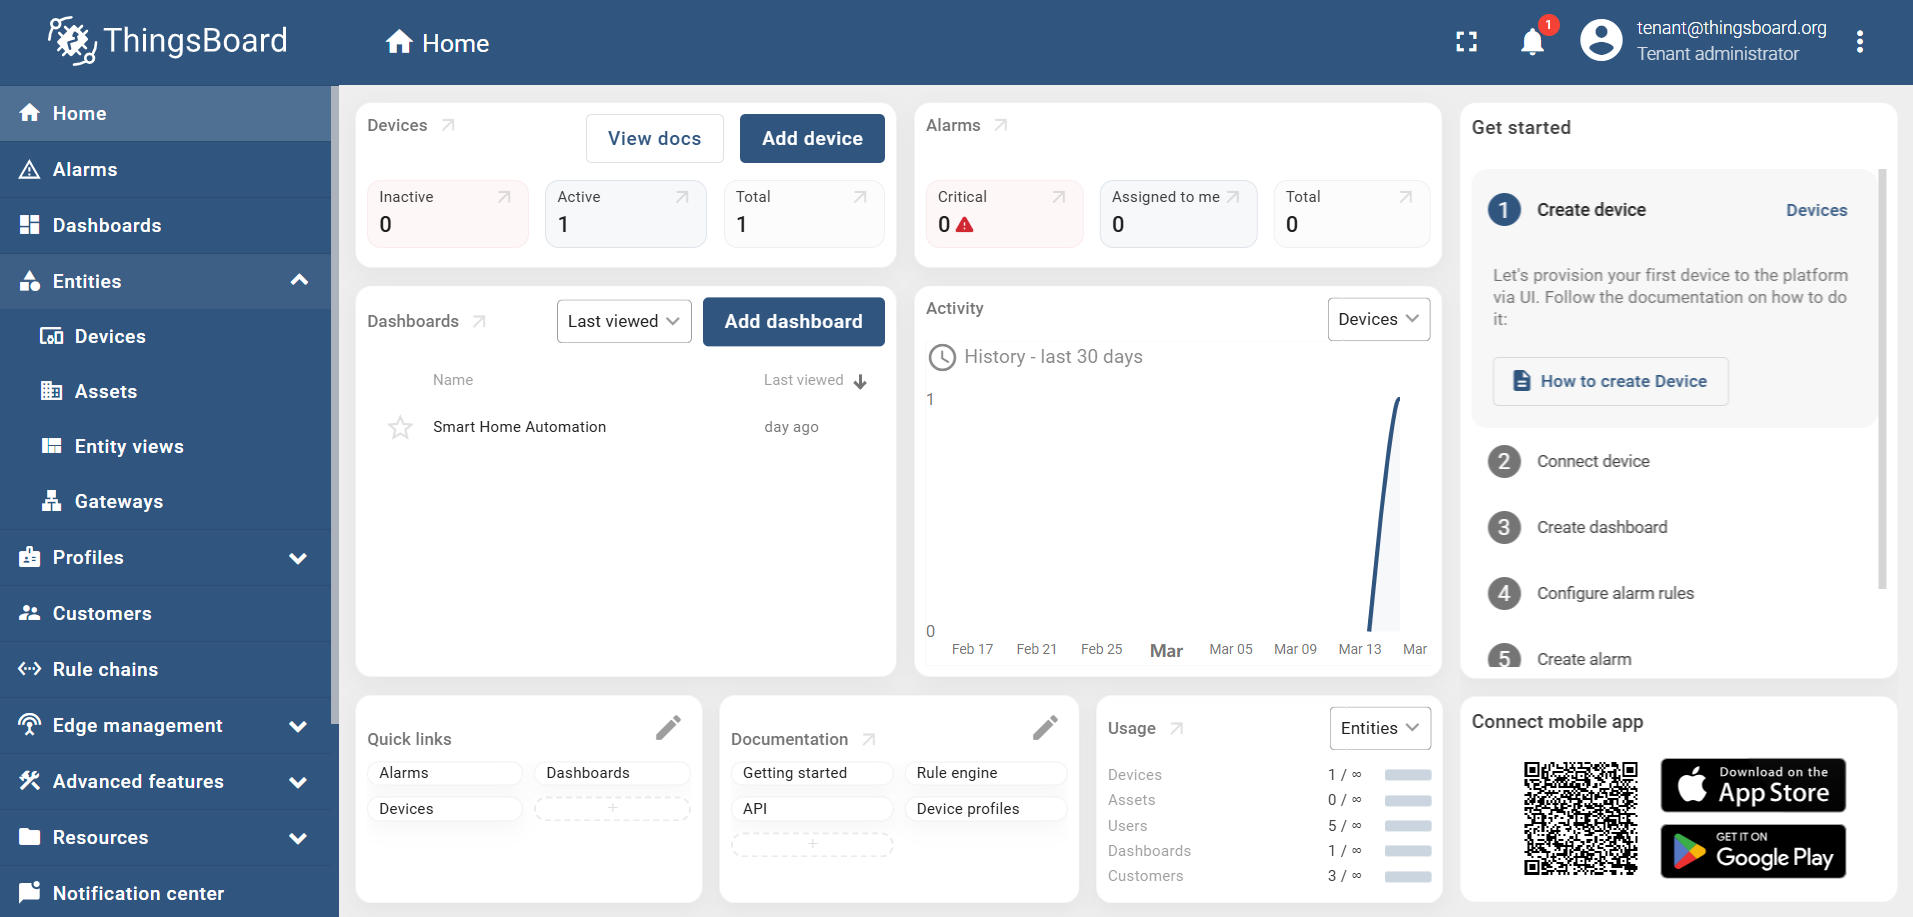
\includegraphics[width=1\textwidth]{home.PNG}
    \caption{ThingsBoard's Home}
 \end{figure}

 \section{Prerequisites for ThingsBoard MQTT Integration}

 Before integrating ThingsBoard with MQTT, ensure that the required software components are installed and configured correctly. The ThingsBoard platform must be running on either a local system or a cloud server. Although ThingsBoard has a built-in MQTT broker, an external broker such as Mosquitto can also be used if needed.Each device must first be created in ThingsBoard before it can communicate via MQTT. To create a new device, navigate to the ThingsBoard dashboard, go to the \textbf{Devices} section, and click on \textbf{Add New Device}. Assign a meaningful name and select the appropriate device type. Once the device is created, an \textbf{Access Token} is generated, which will be required for authentication in MQTT communication. A visual representation of the device creation process is shown in Figure~\ref{fig:device_creation}. Additionally, MQTT communication requires appropriate network settings. Ensure that port \textbf{1883} is open for unencrypted communication. Each device must authenticate with ThingsBoard using an \textbf{Access Token}, which is assigned when the device is created in ThingsBoard.
 
 \begin{figure}[H]
    \centering
    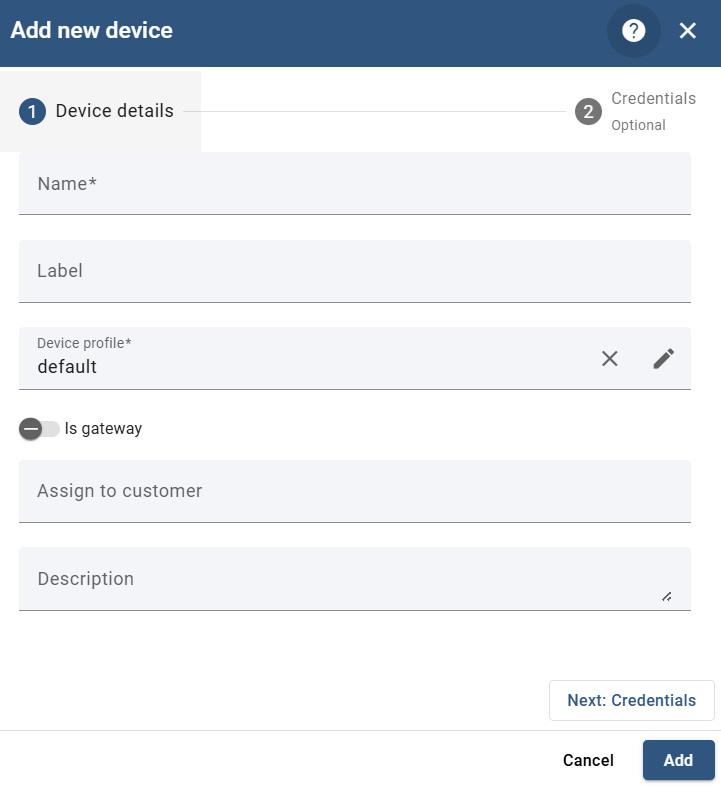
\includegraphics[width=0.35\textwidth]{device creation.PNG}
    \caption{Device creation process in ThingsBoard}
    \label{fig:device_creation}
 \end{figure}

 
 \section{Connecting ThingsBoard with MQTT}
 
 To send telemetry data to ThingsBoard using MQTT, follow these steps:
 
 \subsection{Step 1: Define Connection Parameters}
 The first step is to configure the MQTT connection by specifying the ThingsBoard host, access token, and MQTT port. Replace the \texttt{ACCESS\_TOKEN} with the token obtained from the ThingsBoard device.
 
 \begin{lstlisting}[caption={Connection Parameters as Environment Variables}]
 THINGSBOARD_HOST = "localhost"
 ACCESS_TOKEN = "dU6S0YIAPX5WwfmB3wUi"  # Replace with your actual token
 MQTT_PORT = 1883
 \end{lstlisting}
 
 \subsection{Step 2: Install and Import MQTT Library}
 After setting up the connection parameters, ensure that the \texttt{paho-mqtt} library is installed. This library is required to establish an MQTT connection. Once installed, import the necessary modules in the Python script.
 
 \begin{lstlisting}[caption={Importing MQTT using Python}]
 import paho.mqtt.client as mqtt
 import json
 \end{lstlisting}
 
 \subsection{Step 3: Create MQTT Client and Connect}
 The next step is to create an MQTT client instance and authenticate using the access token. The client must then connect to the ThingsBoard host on the specified port.
 
 \begin{lstlisting}[caption={Connecting MQTT to ThingsBoard using Device Token}]
 client = mqtt.Client()
 client.username_pw_set(ACCESS_TOKEN)  # Use Access Token for authentication
 client.connect(THINGSBOARD_HOST, MQTT_PORT, 60)
 \end{lstlisting}
 
 \subsection{Step 4: Publish Sensor Data}
 Once connected, sensor data must be prepared in JSON format and published to the ThingsBoard MQTT topic. The following code snippet demonstrates how to send temperature and humidity data.
 
 \begin{lstlisting}[caption={Sending Telemetry Response in JSON}]
 telemetry_data = {"current": 14.919, "fan_status": 0,"gas_detected":0,"light":61,"motion":1,"power":3493.48,"power_factor":0.98,"temperature":27.85}
 client.publish("v1/devices/me/telemetry", json.dumps(telemetry_data))
 print("Data sent successfully!")
 client.disconnect()
 \end{lstlisting}

 \begin{figure}[H]
    \centering
    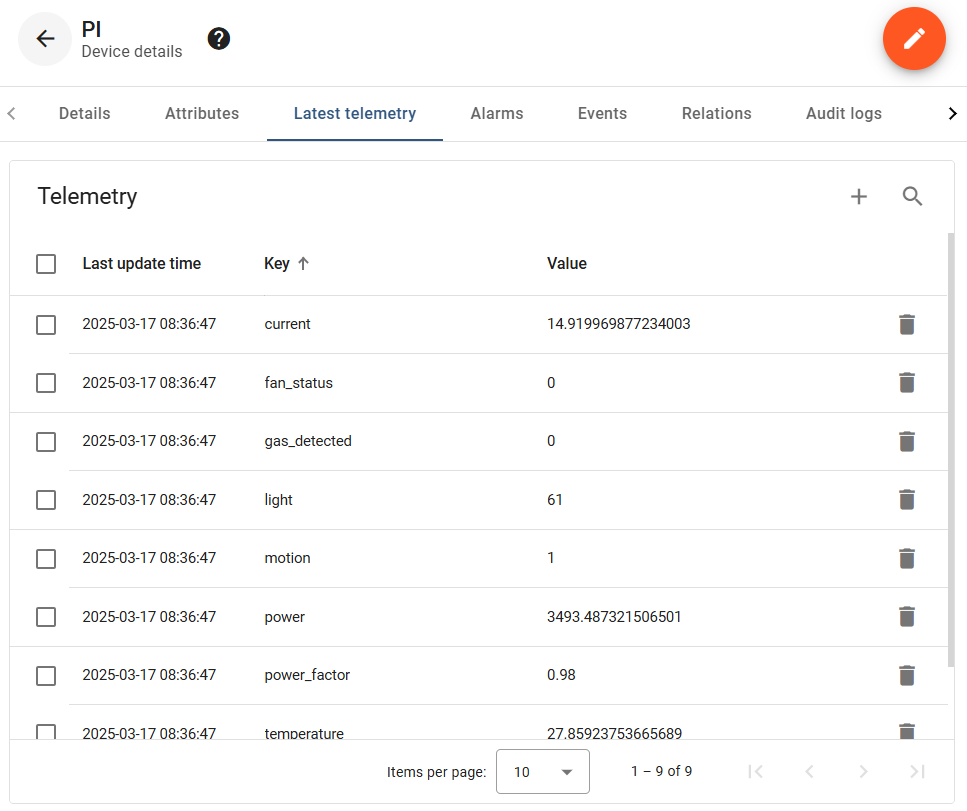
\includegraphics[width=0.8\textwidth]{device Details.PNG}
    \caption{Latest Telemetry after Publishing Data}
 \end{figure}
 
 \subsection{Step 5: Verify Data in ThingsBoard}
 After publishing the data, it is essential to verify whether ThingsBoard has received it. This can be done by navigating to the ThingsBoard UI and checking the \textbf{Latest Telemetry} section of the configured device.

 \subsection{Step 6:Creation of Dashboard in ThingsBoard}
 After creating a device in ThingsBoard, the next step is to create a dashboard for monitoring and visualization. To create a new dashboard, navigate to the \textbf{Dashboards} section and click on \textbf{Create New Dashboard}. Provide a meaningful name and description for easy identification.

 Once the dashboard is created, widgets can be added to visualize device telemetry data. Click on \textbf{Edit Dashboard}, then use the \textbf{Add New Widget} option to select an appropriate widget type, such as charts, gauges, or tables. Link the widget to the corresponding device and telemetry keys. The dashboard creation process is illustrated in Figure~\ref{fig:dashboard_creation2}.
 \begin{figure}[H]
    \centering
    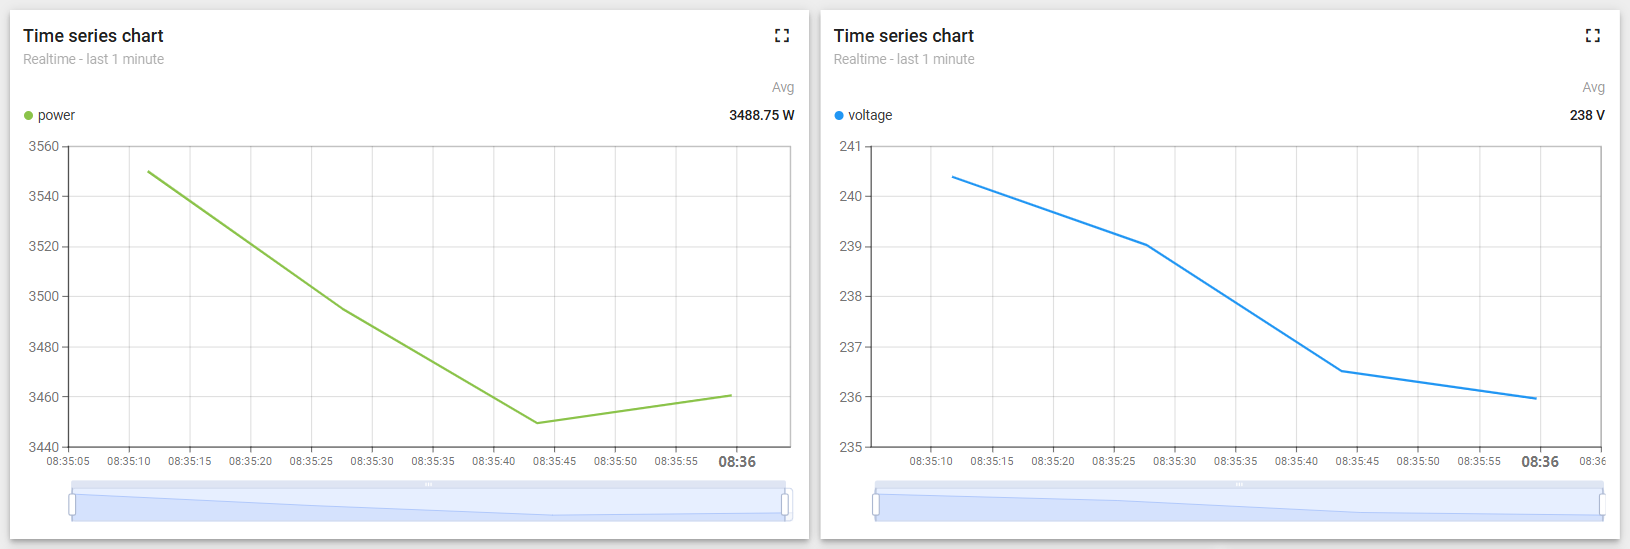
\includegraphics[width=1\textwidth]{dashboard2.PNG}
 \end{figure}
 \begin{figure}[H]
    \centering
    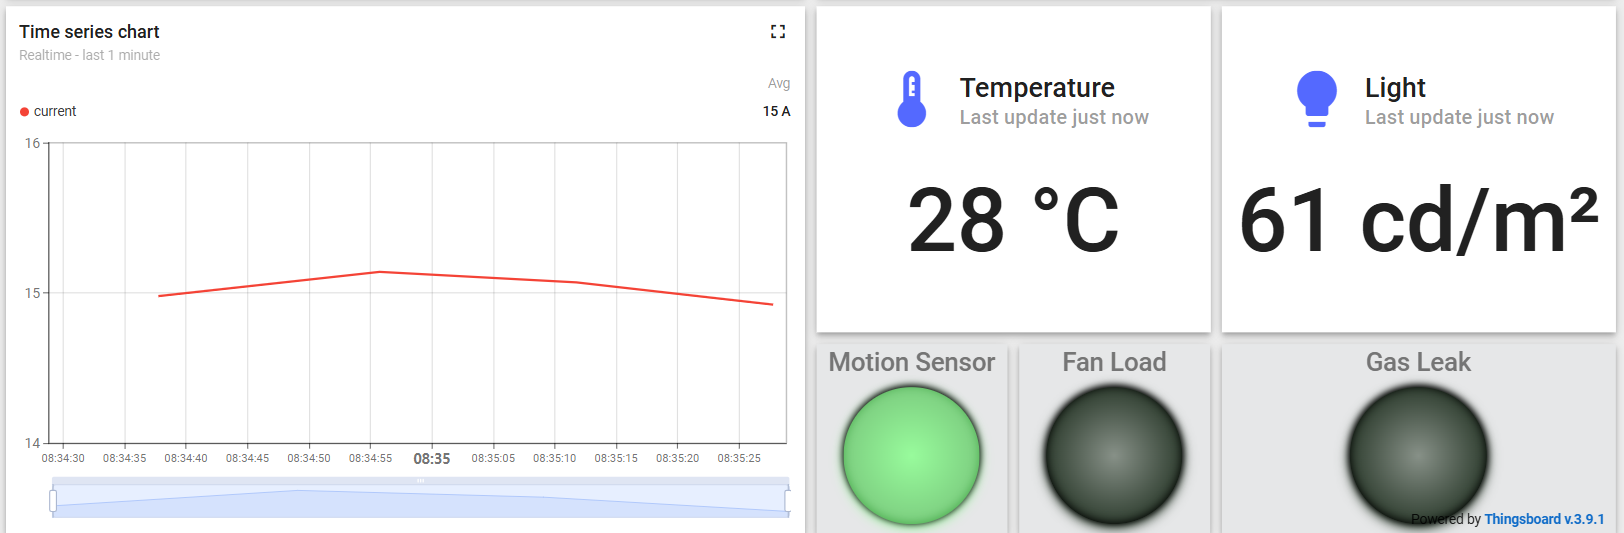
\includegraphics[width=1\textwidth]{dashboard1.PNG}
    \caption{Dashboard Creation with ThingsBoard Widgets}
    \label{fig:dashboard_creation2}
 \end{figure}
 \section{Prerequisites for ThingsBoard API Integration}
 
 Before integrating ThingsBoard with the API, ensure that the required software and authentication mechanisms are set up properly. The ThingsBoard platform must be installed on a local system or a cloud server to facilitate communication. A REST client such as Postman or the \texttt{fetch} API in JavaScript is necessary for interacting with ThingsBoard’s API. Additionally, proper network access should be configured to allow API requests.
 
 To ensure security, ThingsBoard requires authentication via a JSON Web Token (JWT). The authentication process involves sending a username and password to ThingsBoard’s login API. Upon successful authentication, a token is generated, which must be included in all subsequent API requests. Without this token, ThingsBoard will deny access to its resources.
 
 \section{Connecting to ThingsBoard API}
 
 To fetch telemetry data from ThingsBoard, follow these steps:
 
 \subsection{Step 1: Generate Access Token}
 The first step is to authenticate with ThingsBoard and obtain an access token. This is done by sending a POST request to the authentication API with valid credentials. The request should be formatted in JSON, containing a username and password.
 
 \begin{lstlisting}[caption={Content for Body of POST Request}]
 POST http://localhost:9090/api/auth/login
 Content-Type: application/json
 
 {
     "username": "tenant@thingsboard.org",
     "password": "tenant"
 }
 \end{lstlisting}
 
 \subsection{Step 2: Extract JWT Token}
 Once the authentication request is processed, the API will return a response containing a JWT token. This token is essential for making authorized requests to ThingsBoard. The response will be in JSON format, and the token can be extracted from the \texttt{token} field.
 
 \begin{lstlisting}[caption={Response of POST Request}]
 {
     "token": "eyJhbGciOiJIUzI1NiIsInR5cCI...",
     "refreshToken": "eyJhbGciOiJIUzI1NiIsIn..."
 }
 \end{lstlisting}
 
 \subsection{Step 3: Fetch Telemetry Data}
 After obtaining the authentication token, the next step is to retrieve telemetry data from a specific device. The device ID must be specified in the request URL, and the JWT token must be included in the request headers under the \texttt{X-Authorization} field. The following JavaScript code demonstrates how to fetch power telemetry data from a ThingsBoard device.
 
 \begin{lstlisting}[caption={Fetching Data from ThingsBoard using Token Authentication method}]
 const response = await fetch( 
     `http://localhost:9090/api/plugins/telemetry/DEVICE/0eb8ae80-ffe6-11ef-b36a-71656502eb9c/values/timeseries?keys=power`,
     {
         headers: { "X-Authorization": `Bearer ${thingsboardToken}` },
     }
 );
 const data = await response.json();
 console.log(data);
 \end{lstlisting}
 
 \subsection{Step 4: Process Response Data}
 Once the telemetry data is retrieved, it will be returned in JSON format. The response will contain key-value pairs representing the requested telemetry values. The received data can then be processed, displayed, or stored as needed, depending on the application requirements.
 \section{Conclusion}
 Integrating ThingsBoard with MQTT allows for efficient and secure real-time data transmission for IoT devices. By following the methods mentioned, devices can authenticate, publish telemetry data, and take advantage of ThingsBoard's monitoring and automation capabilities. This lightweight and scalable strategy improves IoT installations by providing consistent connectivity while also allowing for future enhancements such as encryption and improved data handling.

 \chapter{Blockchain and Smart Contracts}

 \section{Introduction}
 Blockchain is a decentralized, transparent, and secure technology for managing digital transactions. It combines cryptography, peer-to-peer networks, and consensus mechanisms to ensure that data is immutable and fraud-resistant\cite{swan2016blockchain}\cite{tern2021survey}.Smart contracts, introduced by Ethereum in 2013, are self-executing contracts with code-defined terms. These remove the need for intermediaries and allow for efficient and secure automation of processes in industries such as finance, energy, and logistics\cite{yuan2018shadoweth}\cite{falazi2020smart}\cite{johari2021smart}.
 
 \section{Advantages}
 Blockchain enables decentralization, immutability, and transparency.  Its distributed architecture eliminates single points of failure and enables tamper-proof, cryptographically secure data.  Smart contracts increase efficiency by enforcing logic directly on-chain, decreasing dependency on third parties.
 
 \section{Smart Contract Deployed in the Project}
 The following Solidity contract was deployed to implement a decentralized energy billing system:
 
 \begin{lstlisting}
 // SPDX-License-Identifier: MIT
 pragma solidity ^0.8.0;
 
 contract EnergyBilling {
     address public owner;
     mapping(address => uint256) public userEnergy;
     mapping(address => uint256) public userBills;
 
     uint256 public constant RATE_PER_KWH = 2;
 
     event EnergyStored(address indexed user, uint256 energy);
     event BillPaid(address indexed user, uint256 amount);
 
     modifier onlyOwner() {
         require(msg.sender == owner, "Only owner can call this function");
         _;
     }
 
     constructor() {
         owner = msg.sender;
     }
 
     function storeEnergy(uint256 _totalEnergy) public {
         require(_totalEnergy > 0, "Energy must be greater than zero");
 
         userEnergy[msg.sender] += _totalEnergy;
         userBills[msg.sender] = userEnergy[msg.sender] * RATE_PER_KWH;
 
         emit EnergyStored(msg.sender, _totalEnergy);
     }
 
     function getBill() public view returns (uint256) {
         return userBills[msg.sender];
     }
 
     function payBill() public payable {
         uint256 billAmount = userBills[msg.sender];
         require(msg.value == billAmount, "Incorrect payment amount");
 
         userBills[msg.sender] = 0;
 
         emit BillPaid(msg.sender, msg.value);
     }
 }
 \end{lstlisting}
 
 \section{Web3 Application Setup}
 The frontend for interacting with this contract was built using React and Web3.js. The initial setup was done using Vite:
 
 \begin{lstlisting}
 npm create vite@latest web3-app --template react
 cd web3-app
 npm install
 npm install web3 dotenv
 \end{lstlisting}
 
 \section{Blockchain Connection and Data Interaction}
 A Web3 connection to the smart contract was established using the following code snippet:
 
 \begin{lstlisting}
 import Web3 from "web3";
 
 const web3 = new Web3(import.meta.env.VITE_GANACHE_RPC);
 const contractAddress = import.meta.env.VITE_CONTRACT_ADDRESS;
 const privateKey = import.meta.env.VITE_PRIVATE_KEY;
 const account = import.meta.env.VITE_ACCOUNT;
 \end{lstlisting}
 
 Energy data is fetched from ThingsBoard:
 
 \begin{lstlisting}
 async function fetchEnergyData() {
     const response = await fetch(
         `http://localhost:9090/api/plugins/telemetry/DEVICE/${DEVICE_ID}/values/timeseries?keys=power`,
         { headers: { "X-Authorization": `Bearer ${thingsboardToken}` } }
     );
     const data = await response.json();
     const power = data.power[0].value;
     setEnergy(Math.floor(power));
 }
 \end{lstlisting}
 
 \section{Smart Contract Interaction}
 
 \subsection{Store Energy}
 \begin{lstlisting}
 async function sendEnergyData() {
     const tx = contract.methods.storeEnergy(energy);
     const gas = await tx.estimateGas({ from: account });
     const gasPrice = await web3.eth.getGasPrice();
     const data = tx.encodeABI();
     const nonce = await web3.eth.getTransactionCount(account, "latest");
 
     const signedTx = await web3.eth.accounts.signTransaction(
         { to: contractAddress, data, gas, gasPrice, nonce },
         privateKey
     );
 
     await web3.eth.sendSignedTransaction(signedTx.rawTransaction);
 }
 \end{lstlisting}
 
 \subsection{Fetch and Pay Bill}
 \begin{lstlisting}
 async function fetchBill() {
     const billAmount = await contract.methods.getBill().call({ from: account });
     setBill(billAmount);
 }
 
 async function payBill() {
     const billAmount = await contract.methods.getBill().call({ from: account });
     const tx = contract.methods.payBill();
     const gas = await tx.estimateGas({ from: account, value: billAmount });
     const gasPrice = await web3.eth.getGasPrice();
     const data = tx.encodeABI();
     const nonce = await web3.eth.getTransactionCount(account, "latest");
 
     const signedTx = await web3.eth.accounts.signTransaction(
         { to: contractAddress, data, gas, gasPrice, nonce, value: billAmount },
         privateKey
     );
 
     await web3.eth.sendSignedTransaction(signedTx.rawTransaction);
 }
 \end{lstlisting}
 
 \section{Frontend Interface}
 The React frontend allows users to interact with the contract through a simple UI:
 
 \begin{figure}[H]
 \centering
 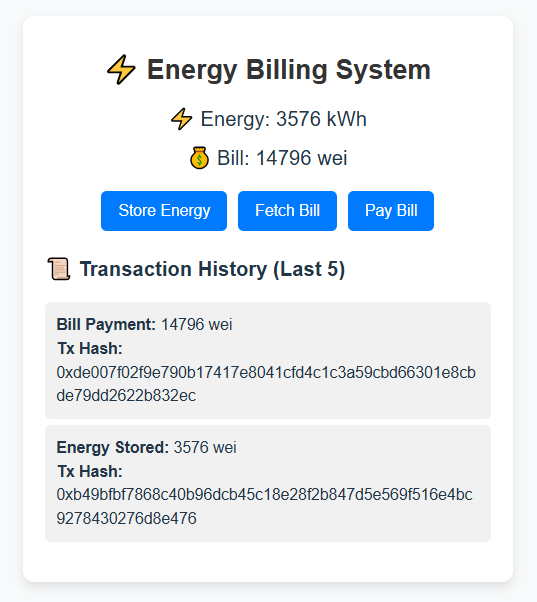
\includegraphics[width=0.4\textwidth]{web3 App.PNG}
 \caption{User interface of the Energy Billing System}
 \label{fig:frontend_ui}
 \end{figure}
 
 \section{Transaction Logs}
 Each smart contract interaction is recorded on the blockchain. The frontend logs these transactions for verification, as shown in Figure~\ref{fig:frontend_transactions}.
 
 \begin{figure}[H]
 \centering
 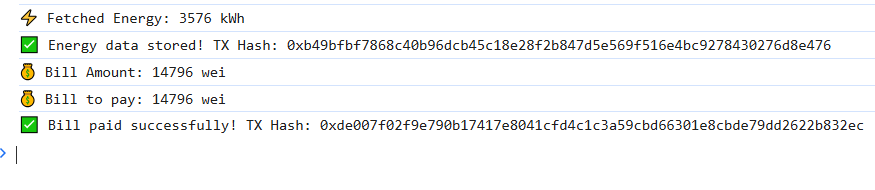
\includegraphics[width=0.8\textwidth]{frontend Logs.PNG}
 \caption{Transaction log from frontend interactions with the smart contract}
 \label{fig:frontend_transactions}
 \end{figure}
 
 \section{Conclusion}
 This chapter demonstrated how blockchain and smart contracts can automate energy billing with transparency and security. By integrating Web3.js, React, and ThingsBoard, a decentralized billing system was developed that showcases the capabilities of Web3 in real-world applications.
 
 \chapter{Conclusion and Future Scope}

This study highlights how combining IoT and smart energy management with home automation may revolutionize energy use, monitoring, and billing.  The system uses real-time data and automation to assure transparency, efficiency, and accuracy in energy monitoring and invoicing, making energy management more streamlined and cost-effective.
 
Building on this foundation, the suggested smart home automation system can be greatly improved by using new technology.  One interesting possibility is the integration of smart grid capabilities, which allows households to exchange excess solar energy within a local network.  This peer-to-peer energy sharing approach encourages sustainable living while increasing overall energy efficiency.
 
Additional advances include the implementation of demand-response systems, which alter energy usage based on real-time grid circumstances, resulting in improved load control and less energy waste.  Furthermore, combining solar energy and smart water pumping technologies can help to create a more self-sufficient household ecosystem.  Solar panel monitoring would enable precise assessment of energy generation and automated distribution to home appliances, while intelligent water pumps could regulate consumption based on supply and demand.
 
Another area for improvement is updating the hardware infrastructure.  Switching to more powerful microcontrollers, such as the ESP32 or other IoT-enabled devices, can greatly improve performance.  These devices outperform the Raspberry Pi in terms of computing power, energy consumption, and built-in connection, making them ideal for real-time and scalable IoT applications.
 
 
 


\newpage
% References
\renewcommand{\bibname}{References}

\bibliographystyle{IEEEtran}
\bibliography{references}

\end{document}


